\section*{Math 202A - HW8 - Dan Davison - \texttt{ddavison@berkeley.edu}}
\begin{mdframed}
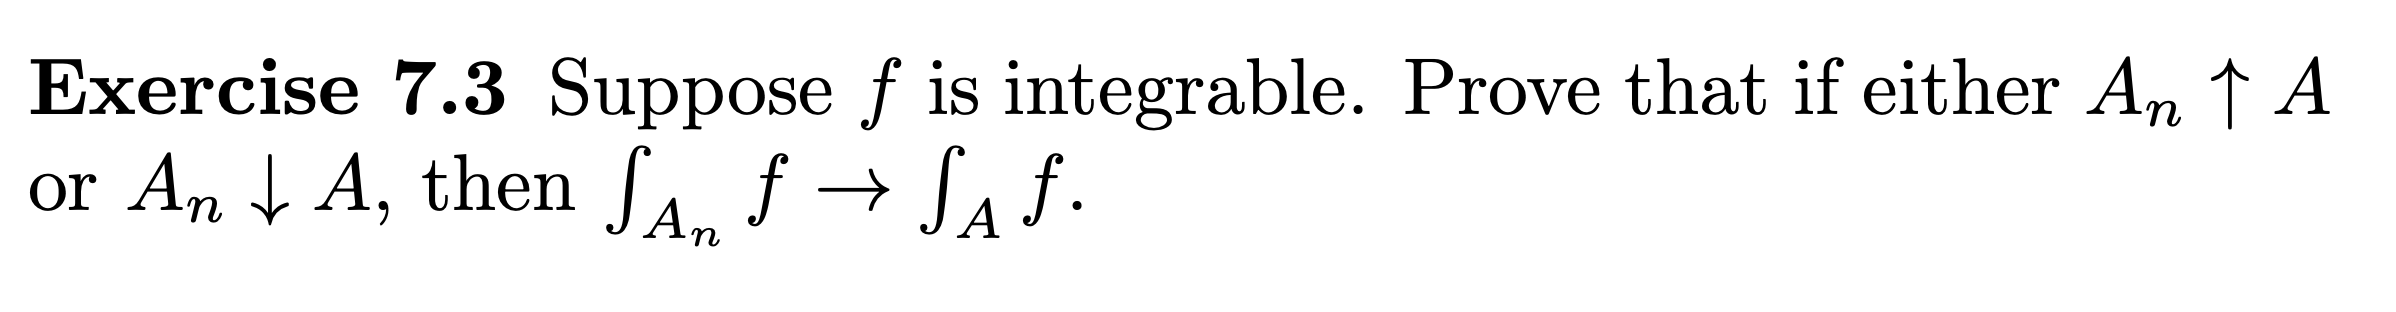
\includegraphics[width=400pt]{img/analysis--berkeley-202a-hw08-2798.png}
\end{mdframed}

\begin{proof}
  The required result is equivalent to
  \begin{align*}
    \limn \int f \ind_{A_n} = \int f \ind_A.
  \end{align*}

  Suppose first that $A_n \uparrow A$.

  Note that
  \begin{align*}
    \limn f\ind_{A_n} = f\limn\ind_{A_n} = f\ind_A,
  \end{align*}
  and furthermore that $|f\ind_{A_n}| \leq f$ for all $n$ and $f$ is integrable. Therefore by the dominated
  convergence theorem we have
  \begin{align*}
    \limn \int f \ind_{A_n} = \int f \ind_A,
  \end{align*}
  as required.

  Next suppose that $A_n \downarrow A$. Thus $A_n \supseteq A$ for all $n$, and $A_n^c \uparrow A^c$. In
  parallel with the previous argument we have
  \begin{align*}
    \limn f\ind_{A_n^c} = f\limn\ind_{A_n^c} = f\ind_{A^c},
  \end{align*}
  and furthermore $|f\ind_{A_n^c}| \leq f$ for all $n$ and $f$ is integrable.  Therefore by the dominated
  convergence theorem we have
  \begin{align*}
    \limn \int f \ind_{A_n^c} = \int f \ind_{A^c}.
  \end{align*}
  This can be written in terms of integrals over the original (non-complemented) sets as
  \begin{align*}
    \limn \Bigg(\int f - \int f \ind_{A_n}\Bigg) = \int f - \int f \ind_{A},
  \end{align*}
  or equivalently
  \begin{align*}
    \int f - \limn \int f \ind_{A_n} = \int f - \int f \ind_{A}.
  \end{align*}
  Since $\int f < \infty$ we may subtract $\int f$ from both sides, and then multiply by $-1$, yielding
  \begin{align*}
    \limn \int f \ind_{A_n} = \int f \ind_{A},
  \end{align*}
  as required.
\end{proof}

\begin{mdframed}
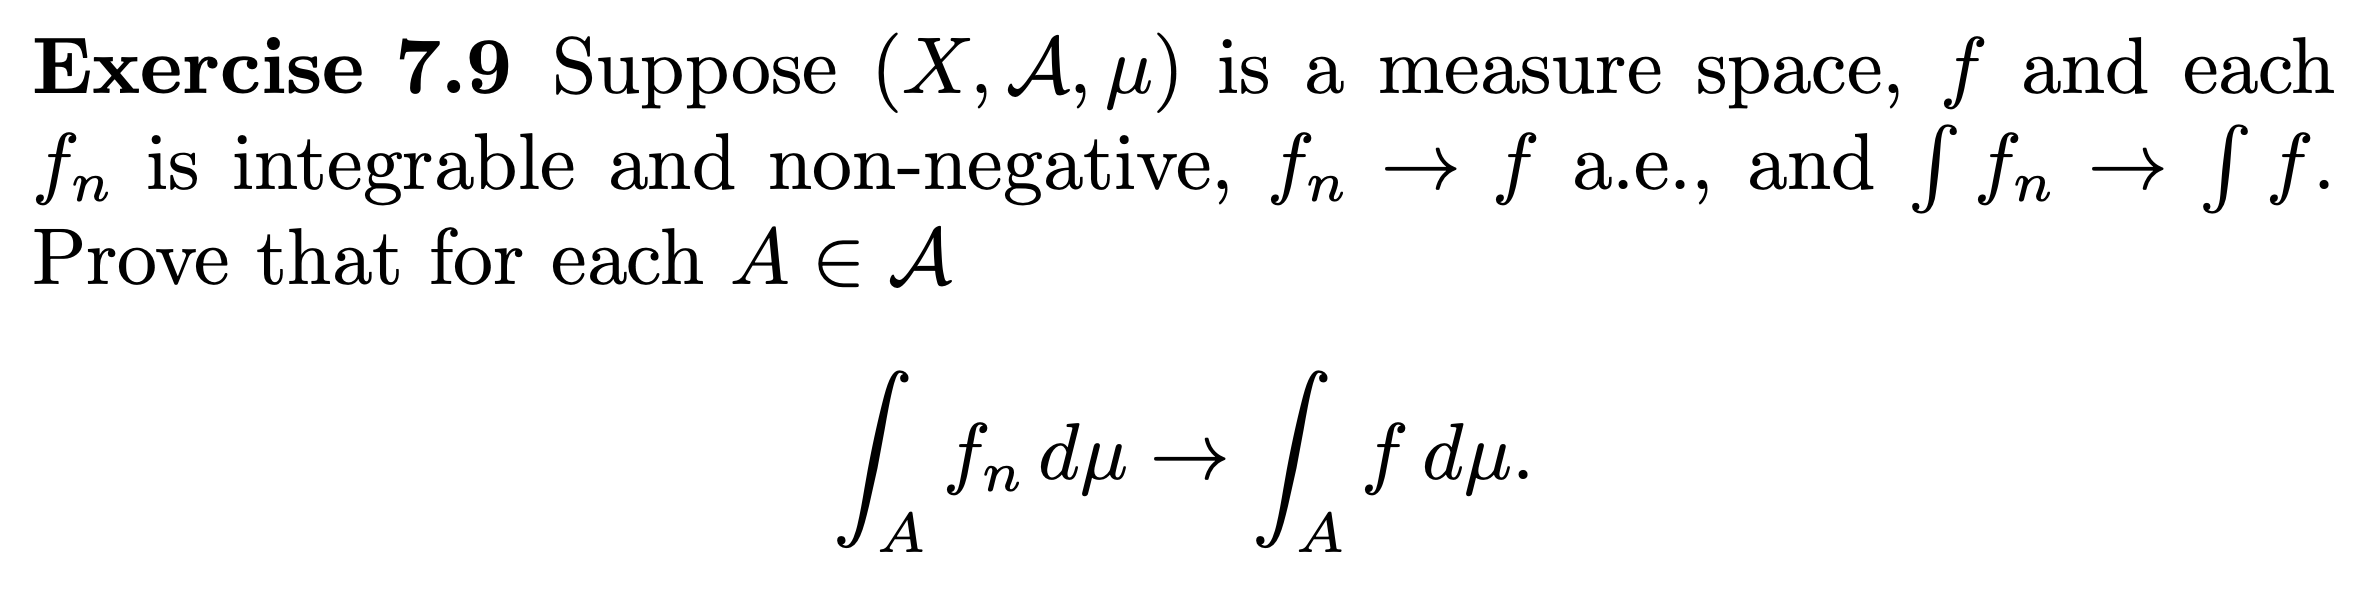
\includegraphics[width=400pt]{img/analysis--berkeley-202a-hw08-3203.png}
\end{mdframed}

\begin{remark*}
  We have that $\int_X f_n \to \int_X f$. What we must show is that this limit-of-integrals still holds when
  the integrals are restricted to $A \subset X$.

  In general, this is not true. For example, let $X = [0, 1]$ and let $f(x) = 0$. Now for odd $n$, let $f_n(x)$
  take the value $-1$ for $0 \leq x < 0.5$ and $+1$ for $0.5 \leq x \leq 1$, and for even $n$ let it take $+1$
  on the first interval and $-1$ on the second. Then $\int_X f_n = 0 = \int_X f$ for all $n$, so the
  hypothesis $\int_X f_n \to \int_X f$ does hold. But $\int_{[0, 0.5]} f_n$ is the
  sequence $-\frac{1}{2}, +\frac{1}{2}, -\frac{1}{2}, \ldots$ and thus has no limit.

  What we need to show is that the result does hold with the additional hypotheses.
\end{remark*}

\begin{proof}
  Let $A \in \mc A$.

  We must show that $\int_A f_n \to \int_A f$.

  We have that $f_n \to f$ a.e. and that $f$ and the $f_n$ are non-negative and integrable, and also
  that $\int_X f_n \to \int_X f$.


  ...


  Since $f_n\ind_{A}$ is a sequence of functions that converge pointwise a.e. to $f\ind_A$,
  with $|f_n\ind_A| < b$ and $b$ is integrable, by the dominated convergence theorem we have
  \begin{align*}
    \int f_n\ind_A \to \int f\ind_A.
  \end{align*}





  Let $g_n = \inf_{m \geq n} f_n$. Then $(g_n)$ is an increasing sequence of functions
  and $g_n \to \liminf_{n \to \infty} f_n = \limn f_n = f$ a.e.

  Then by the MCT we have
  \begin{align*}
    \int g_n \to \int f
  \end{align*}
  How does that help though? We're trying to prove something about $\int f_n$, not about the $\inf$.
  ...





  %%%%%%%%%%%%%%%%%%%%%%%%



  We will find a dominating function and apply the dominated convergence theorem.





  Let $G = \{x \in X ~:~ f_n(x) \to f(x)\}$. Note that $\mu(G) = \mu(X)$.

  We have
  \begin{align*}
    \limn \int_A f_n
    &= \limn \int f_n \ind_{A} \\
    &= \limn \int (f_n \ind_{A \cap G} + f_n \ind_{A \cap (X \setminus G)}) \\
    &= \limn \Bigg(\int f_n \ind_{A \cap G} + \int_{A \cap (X \setminus G)} f_n\Bigg) ~~~~~~~~~~~~~~~~\text{linearity of integral}\\
    &= \limn \int f_n \ind_{A \cap G} ~~~~~~~~~~~~~~~~~~~~~~~~~~~~~~~~~~~~~~~~~~\text{integral over a measure zero set is zero}\\
  \end{align*}
  Note that $f_n\ind_G \to f\ind_G$ pointwise by our definition of $G$.

\end{proof}

\begin{mdframed}
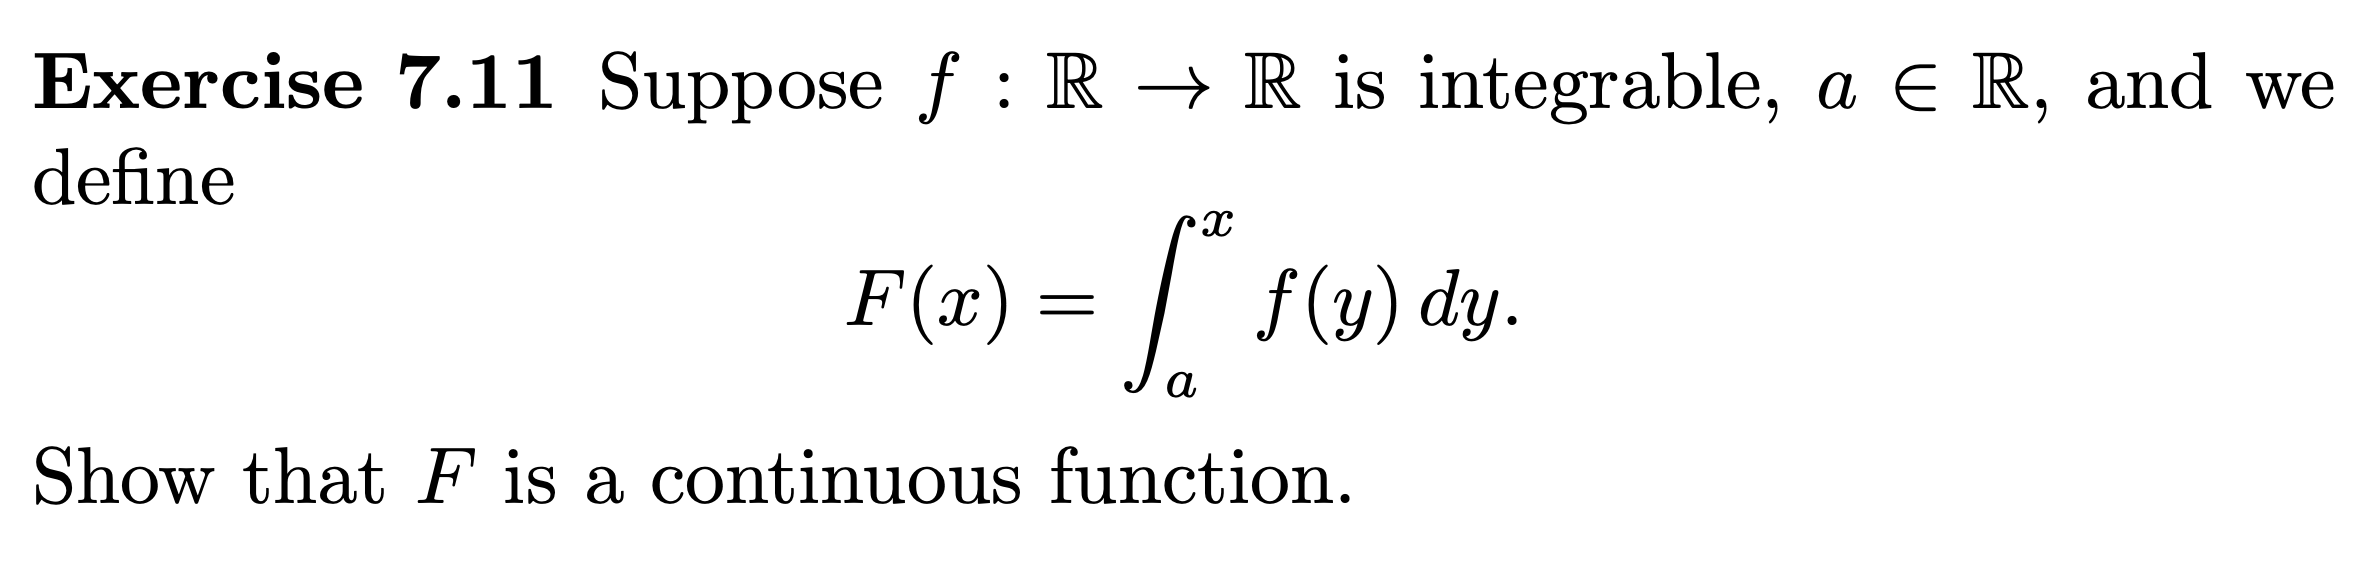
\includegraphics[width=400pt]{img/analysis--berkeley-202a-hw08-d0c0.png}
\end{mdframed}

\begin{mdframed}
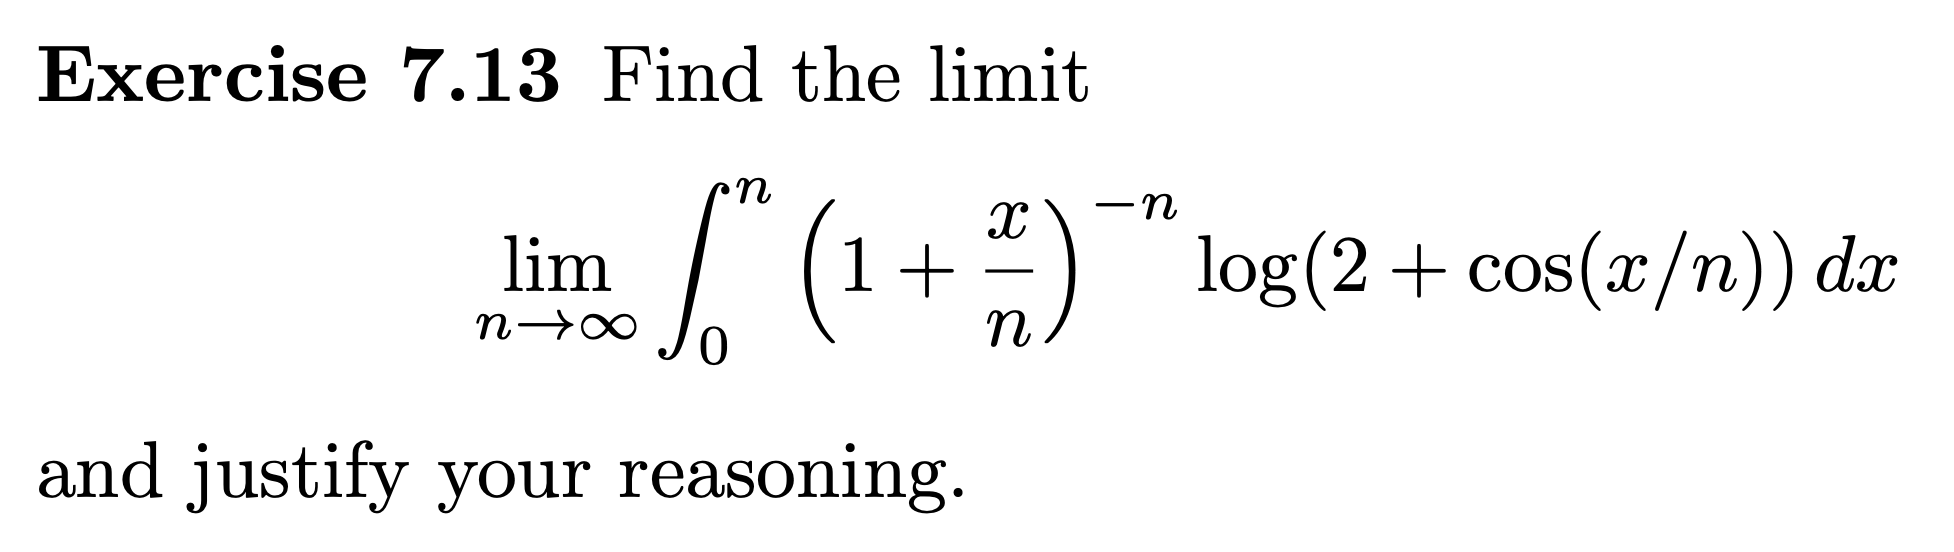
\includegraphics[width=400pt]{img/analysis--berkeley-202a-hw08-9931.png}
\end{mdframed}


\begin{mdframed}
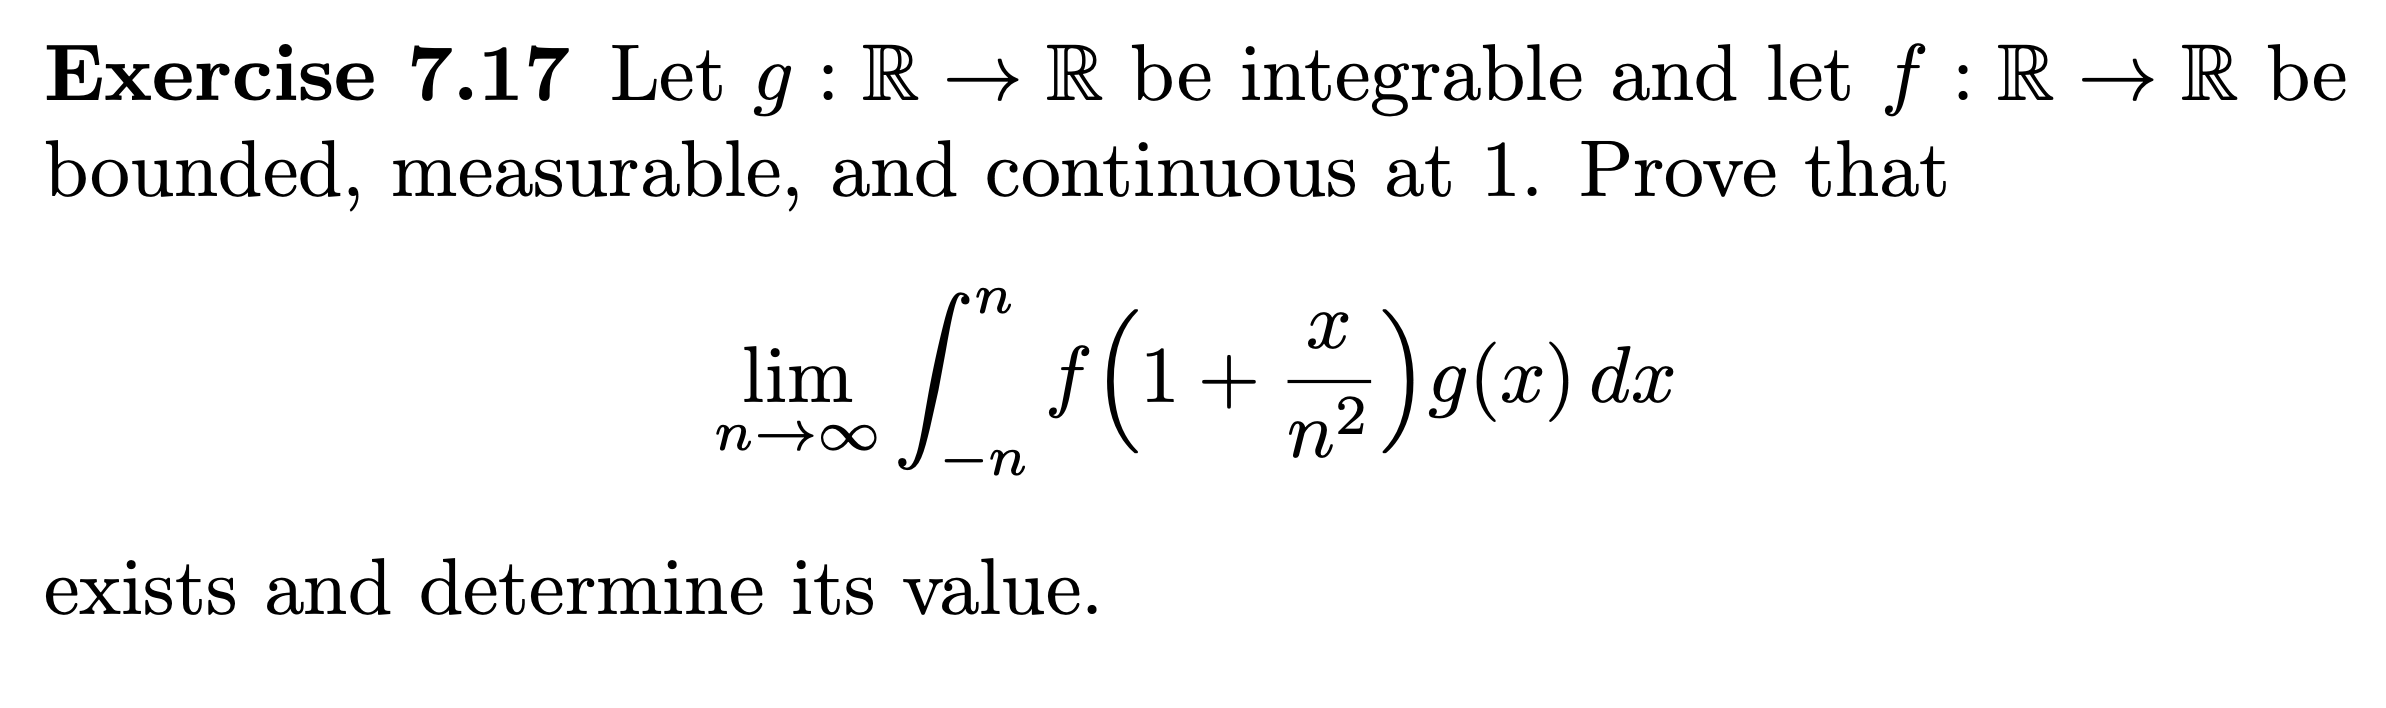
\includegraphics[width=400pt]{img/analysis--berkeley-202a-hw08-6e60.png}
\end{mdframed}


\begin{mdframed}
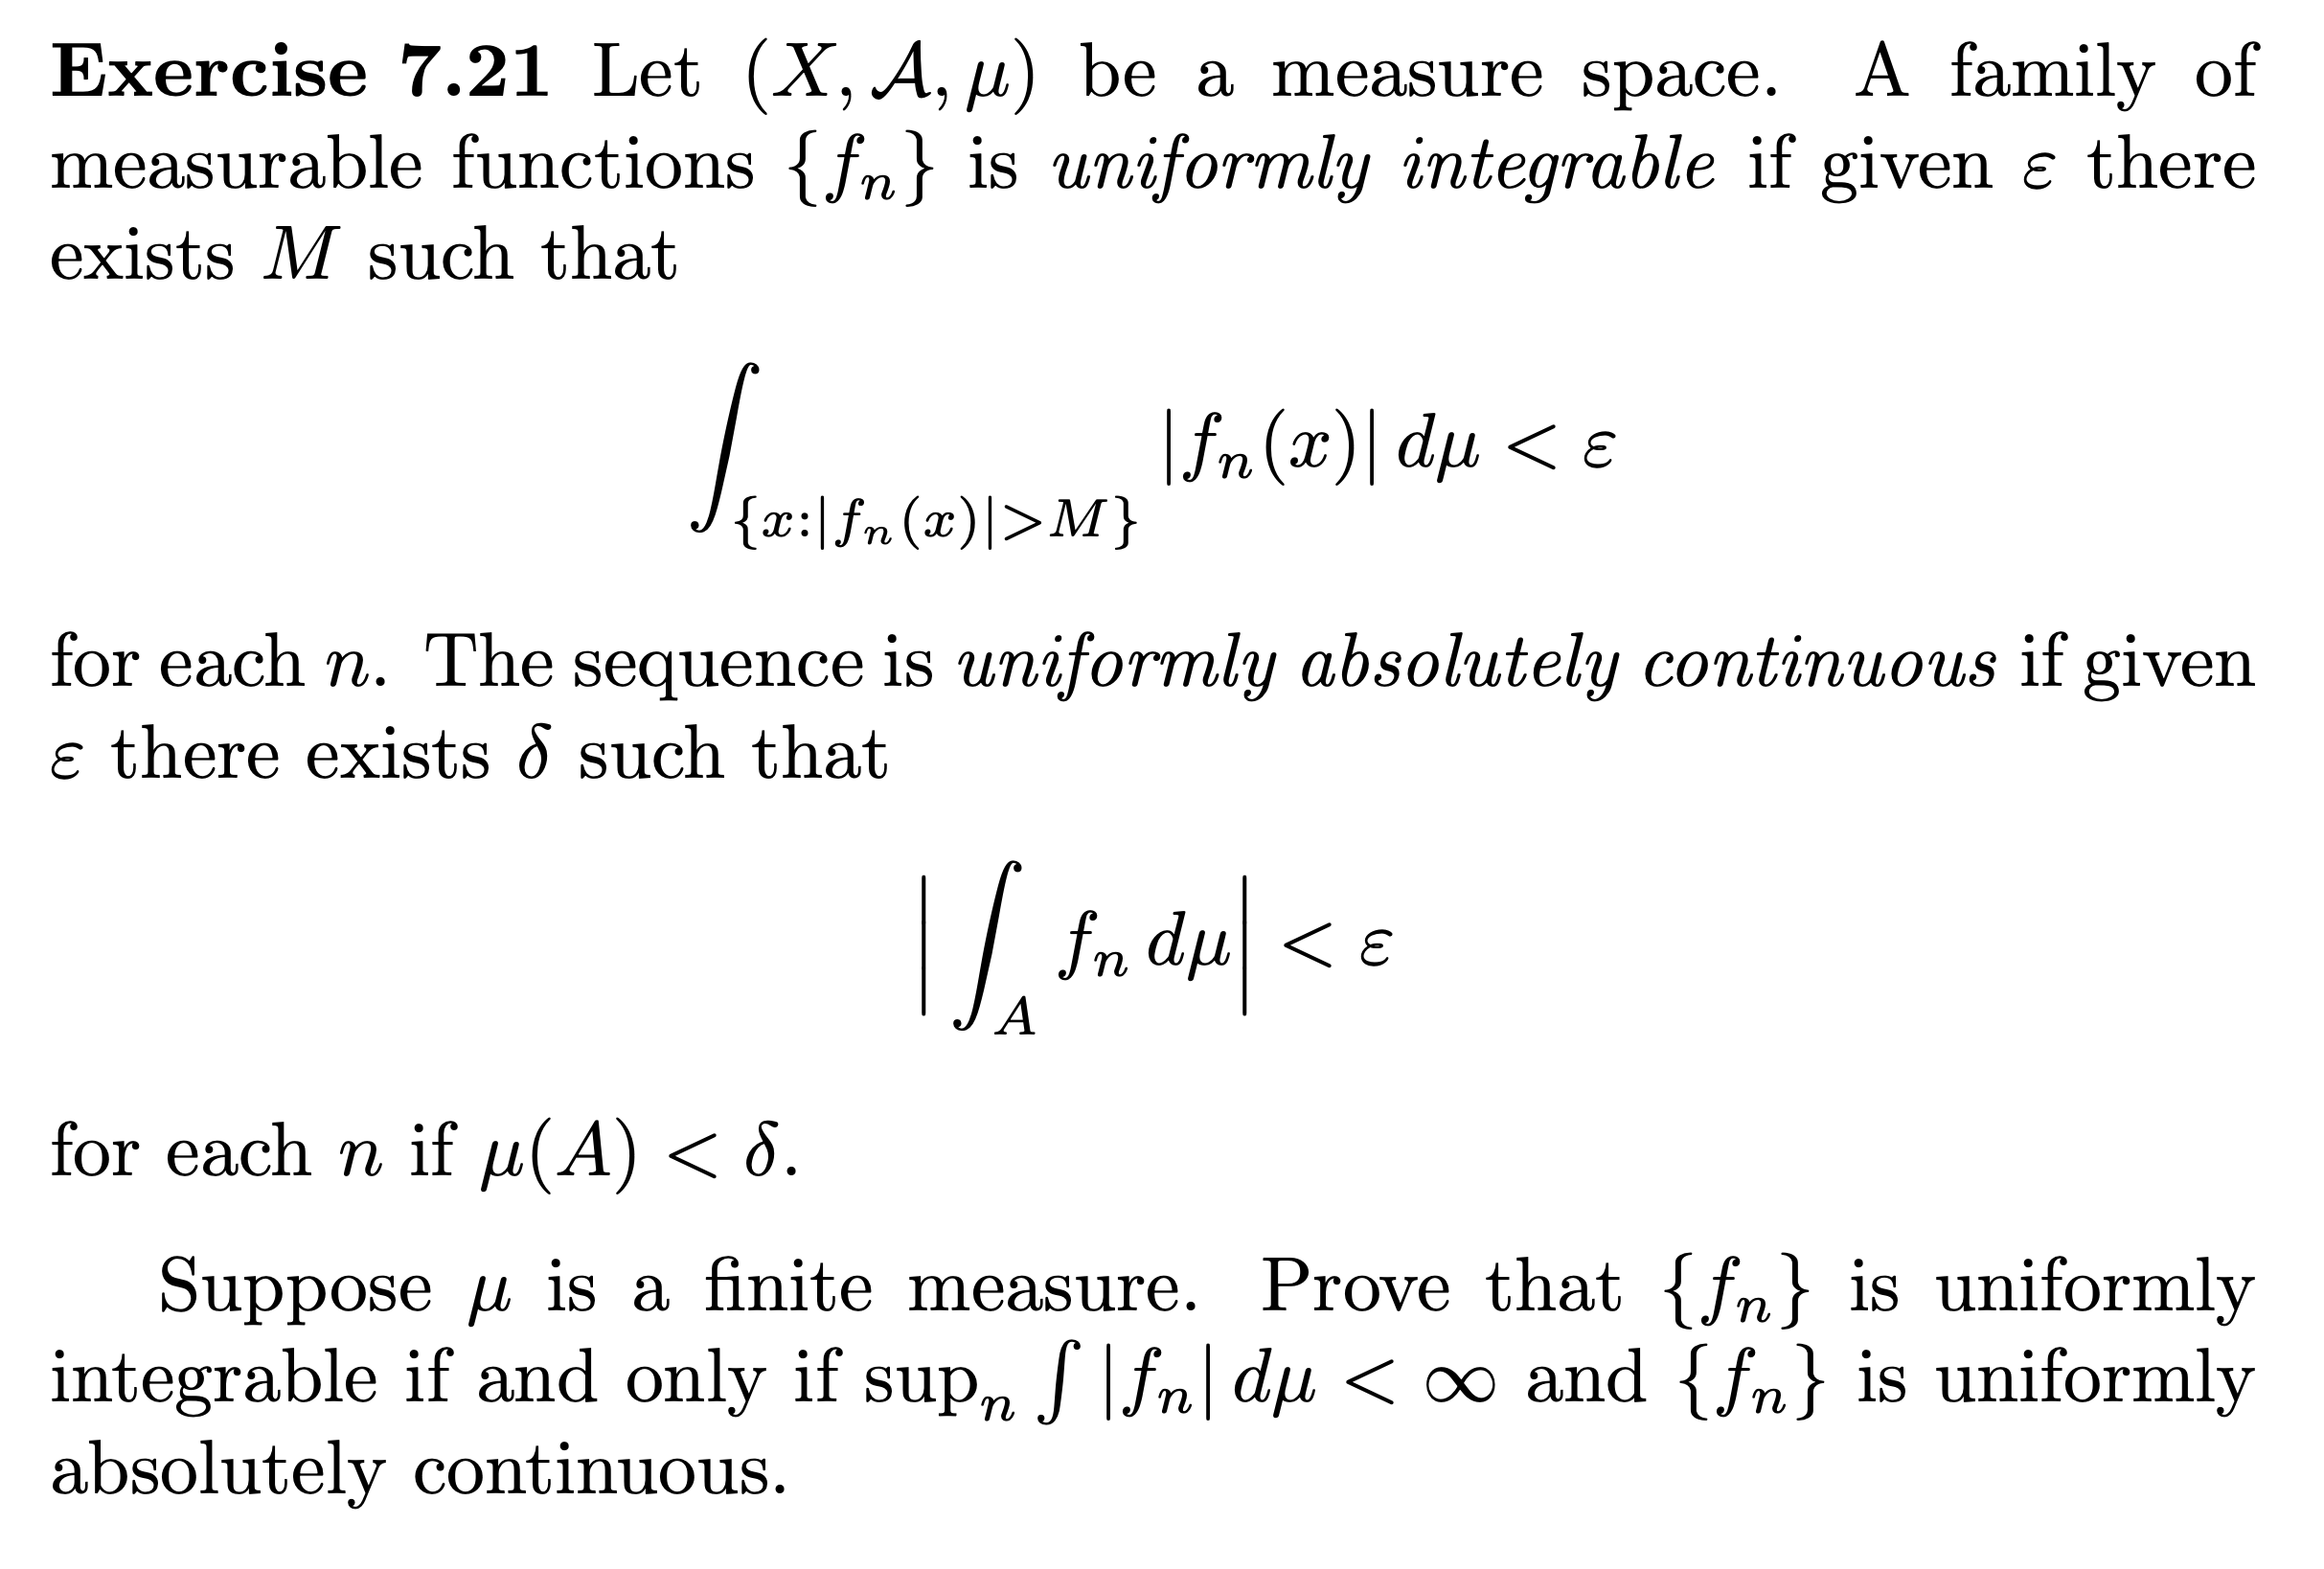
\includegraphics[width=400pt]{img/analysis--berkeley-202a-hw08-337f.png}
\end{mdframed}